\documentclass{beamer}
    \usepackage{../inc/ssbeamer}

    \title{Boids}
    \subtitle{Grupo 01}

    \begin{document}

    \frame{\titlepage}

    \section{Fundamentos}
    \subsection{Algoritmo}
    \begin{frame}
        \frametitle{Boids: Algoritmo}
        \includegraphics[width=\linewidth,height=\textheight,keepaspectratio]{{../imgs/algo_boids}.png}
    \end{frame}
    \subsection{Reglas básicas}
    \begin{frame}
        \frametitle{Boids: Reglas}
        \includegraphics[width=\linewidth,height=\textheight,keepaspectratio]{{../imgs/rules_overview}.png}
    \end{frame}

    \begin{frame}
        \frametitle{Regla: Alineamiento}
        \begin{columns}
            \column{0.7\textwidth}
            \includegraphics[width=\linewidth,height=\textheight,keepaspectratio]{{../imgs/algo_alignment}.png}
            \column{0.3\textwidth}
            \includegraphics[width=\linewidth,height=\textheight,keepaspectratio]{{../imgs/rule_alignment}.png}
        \end{columns}
    \end{frame}

    \begin{frame}
        \frametitle{Regla: Separación}
        \begin{columns}
            \column{0.7\textwidth}
            \includegraphics[width=\linewidth,height=\textheight,keepaspectratio]{{../imgs/algo_separation}.png}
            \column{0.3\textwidth}
            \includegraphics[width=\linewidth,height=\textheight,keepaspectratio]{{../imgs/rule_separation}.png}
        \end{columns}
    \end{frame}

    \begin{frame}
        \frametitle{Regla: Cohesión}
        \begin{columns}
            \column{0.7\textwidth}
            \includegraphics[width=\linewidth,height=\textheight,keepaspectratio]{{../imgs/algo_cohesion}.png}
            \column{0.3\textwidth}
            \includegraphics[width=\linewidth,height=\textheight,keepaspectratio]{{../imgs/rule_cohesion}.png}
        \end{columns}
    \end{frame}
    \subsection{Reglas extendidas}
    \begin{frame}
        \frametitle{Regla: Tendencia a}
        \includegraphics[width=\linewidth,height=\textheight,keepaspectratio]{{../imgs/algo_tendencyto}.png}
    \end{frame}

    \begin{frame}
        \frametitle{Regla: Frontera}
        \begin{center}
        \includegraphics[width=\linewidth,height=0.9\textheight,keepaspectratio]{{../imgs/algo_boundary}.png}
        \end{center}
    \end{frame}

    \section{Implementación}
        \begin{frame}
            \frametitle{Implementación}
            \metroset{block=fill}
            \begin{block}{Lenguaje}
                Kotlin
            \end{block}
            \begin{block}{Avance de simulación y animación}
                $\Delta t = \frac{1}{60}$ (s)
            \end{block}

            \begin{block}{Método de actualización}
                Beeman modificado (fuerza depende de $v_t$)
            \end{block}
        \end{frame}

        \subsection{Código}

        \begin{frame}
            \frametitle{Entidades}
            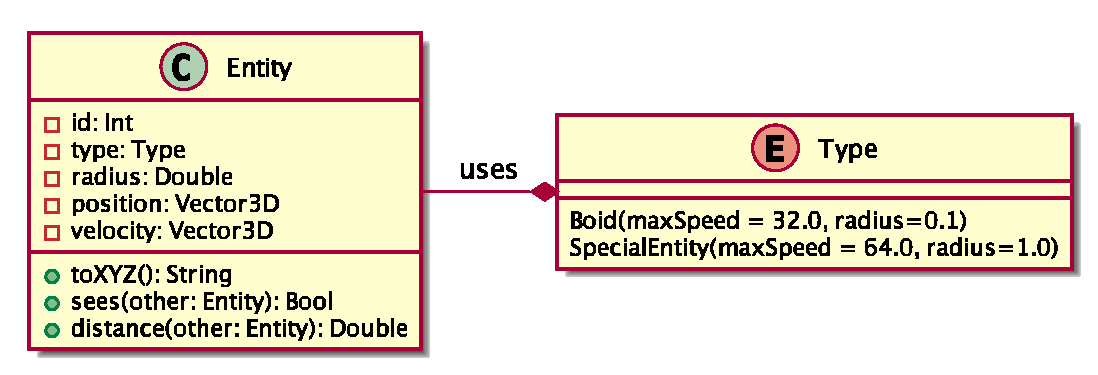
\includegraphics[width=\linewidth,height=\textheight,keepaspectratio]{{../imgs/entity}.eps}
        \end{frame}

        \begin{frame}
            \frametitle{Reglas}
            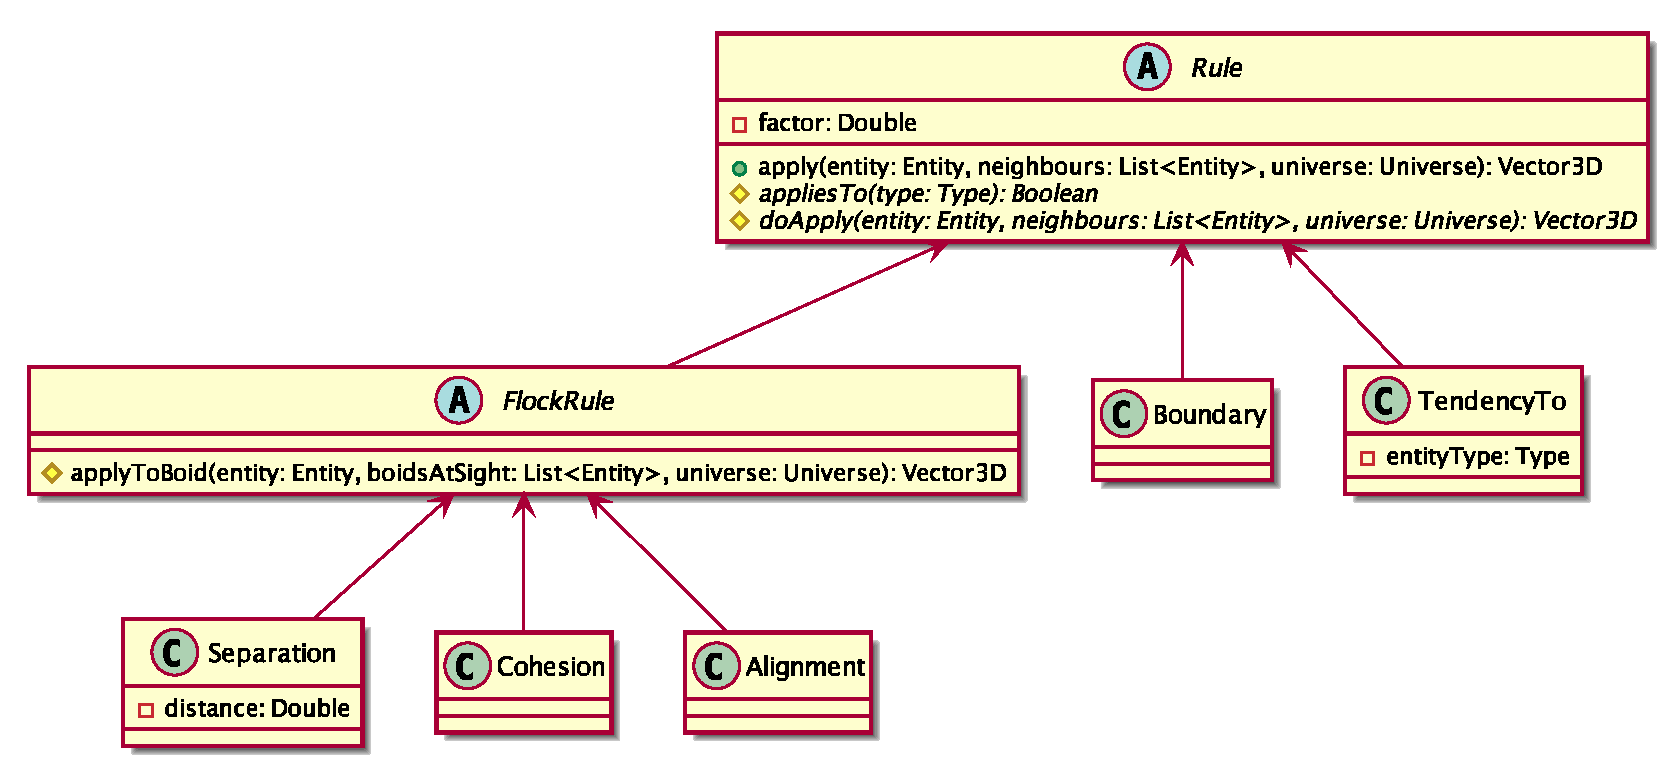
\includegraphics[width=\linewidth,height=\textheight,keepaspectratio]{{../imgs/rules}.eps}
        \end{frame}

        \begin{frame}
            \frametitle{Universo}
            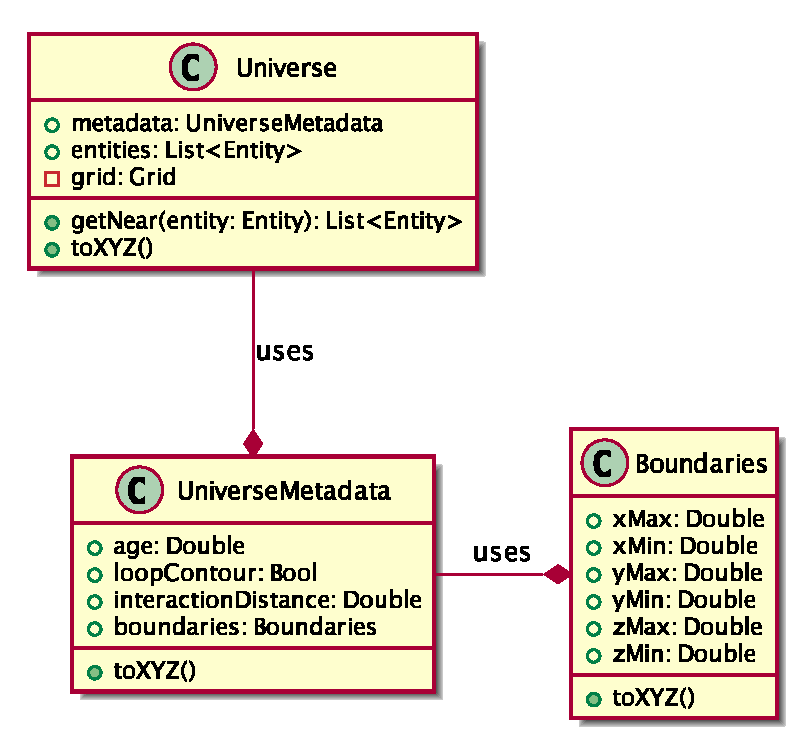
\includegraphics[width=\linewidth,height=\textheight,keepaspectratio]{{../imgs/universe}.eps}
        \end{frame}

        \begin{frame}
            \frametitle{Grilla}
            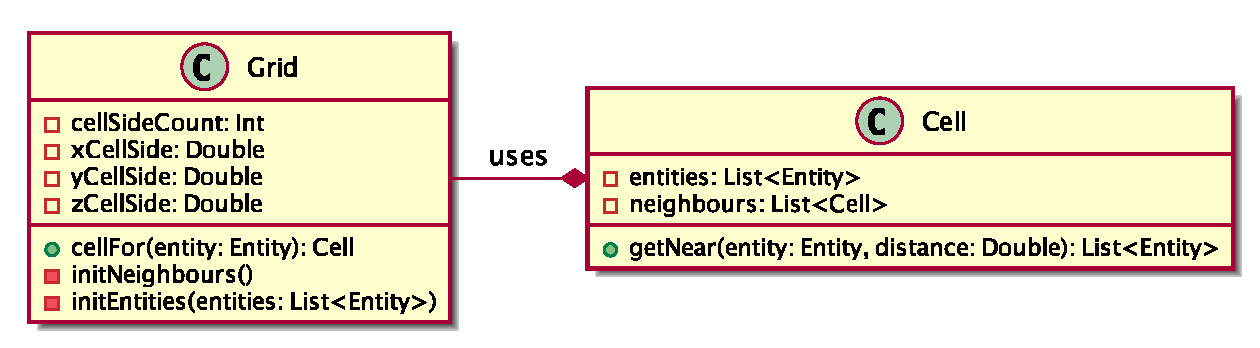
\includegraphics[width=\linewidth,height=\textheight,keepaspectratio]{{../imgs/grid}.eps}
        \end{frame}

        \begin{frame}
            \frametitle{Simulación}
            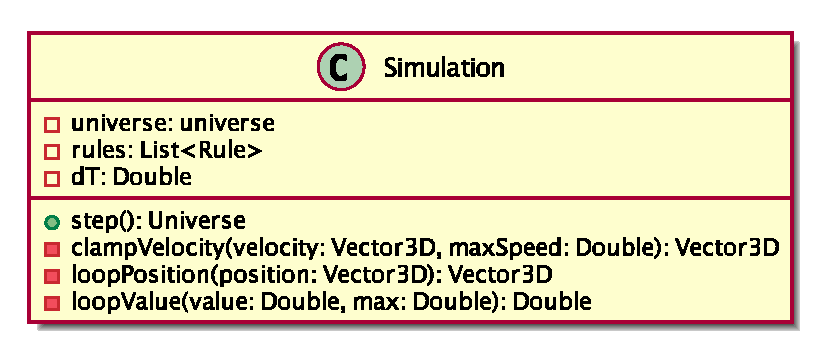
\includegraphics[width=\linewidth,height=\textheight,keepaspectratio]{{../imgs/simulation}.eps}
        \end{frame}
    \section{Resultados}
        \begin{frame}
            \frametitle{Parámetros de simulación}
            \metroset{block=fill}
            \begin{block}{[TODO] Cantidad de personas}
                200
            \end{block}
            \begin{block}{Tamaño del universo}
                20m x 20m x 20m
            \end{block}
            \begin{block}{Radio: boids}
                0.1m
            \end{block}
            \begin{block}{Radio: especiales}
                0.4m
            \end{block}
            \begin{block}{Distancia de interacción}
                3m
            \end{block}
        \end{frame}
    \section{Conclusiones}
    \begin{frame}
        \frametitle{[TODO] Conclusiones}
        \begin{itemize}
            \item TODO
        \end{itemize}
    \end{frame}
    \end{document}
